\chapter{Estudo Experimental de Software}

Este capítulo provê o roteiro de experimentação de software para ferramentas de ETL utilizando dados estruturados, semi estruturados e não estruturados. A Engenharia de Software Experimental tem como objetivo aprimorar métodos, técnicas e ferramentas de Engenharia de Software a partir de métodos experimentais (Isaque Elcio de Souza, TESE - Um sistema de Inf para Geren de Projetos Experimentais em ES). As etapas definidas no processo de experimentação em Engenharia de Software proposto por [Amaral (),Isaque Elcio de Souza, TESE ] consiste em etapas de definição, planejamento, operação, interpretação dos dados e empacotamento que serão melhor detalhados nas seções a seguir.
\clearpage

\section{Objetivos do experimento}

O objetivo principal da aplicação deste experimento é definir se o framework proposto por esta pesquisa de dissertação é uma ferramenta adequada para auxiliar no desenvolvimento de processos de ETL em dados estruturados, semi estruturados e não estruturados.

\subsection{Objetivo da Medição}

Tendo como base as ferramentas de ETL existentes na literatura, caracterizar:

\begin{enumerate}
	\item Quais as principais funcionalidades que as ferramentas de ETL oferecem:
	\begin{enumerate}
		\item essas funcionalidades manipulam dados estruturados, semi estruturados e não estruturados.
		\item  essas funcionalidades não manipulam dados estruturados, semi estruturados e não estruturados.
	\end{enumerate}
	\item Quais funcionalidades podem ser consideradas fundamentais para a produtividade na criação de processos de ETL:
	\begin{enumerate}
		\item quais necessitam manipular dados em grande escala.
		\item quais não manipulam grande volume de dados.
	\end{enumerate}
	\item Quais funcionalidades poderiam aprimorar as ferramentas de ETL.
\end{enumerate}

\subsection{Objetivos do Estudo}

\begin{itemize}
	\item Analisar as ferramentas de ETL para dados estruturados, semi estruturados e não estruturados;
	
	\item Com o propósito de caracterizar;
	
	\item Com respeito à intersecção das ferramentas de ETL existente;
	
	\item Do ponto de vista da literatura;
	
	\item No contexto de comparativo entre as ferramentas mais conhecidas no mercado atual.
\end{itemize}


\subsection{Questões}

Q1. Existem funcionalidades listadas pelas ferramentas pesquisadas que não estão presentes no ETL4NoSQL?

Métrica: A lista de funcionalidades que não estão presentes no ETL4NoSQL.

Q2. Existem funcionalidades oferecidas pelo ETL4NoSQL que não estão presentes nas ferramentas apresentadas pela literatura?

Métrica: A lista de funcionalidades que não estão presentes nas ferramentas da literatura.

Q3. Existem funcionalidades que não estão presentes no ETL4NoSQL e nas ferramentas da literatura que poderiam ser implementadas?

Métrica: A lista de funcionalidades que não estão presentes em nenhuma das ferramentas.

\section{Planejamento}

Na etapa de planejamento são definidas as hipóteses do estudo, a descrição da instrumentação, as métricas, seleção do contexto e dos indivíduos, as variáveis, a análise qualitativa e a validade do experimento. Todas elas serão descritas nas seções seguintes.

\subsection{Definição das Hipóteses}

Hipótese nula (H0): As funcionalidades oferecidas pelo ETL4NoSQL são similares às funcionalidades oferecidas pelas ferramentas presentes na literatura.

Fp - Funcionalidades do ETL4NoSQL

Fl - Funcionalidades das ferramentas da literatura

H0: Fl - (Fp $\cap$ Fl) = $\emptyset$
\newline

Hipótese alternativa (H1): A lista de funcionalidades oferecidas pelo ETL4NoSQL é diferente da lista de funcionalidades oferecidas pelas ferramentas presentes na literatura.

Fp - Funcionalidades do ETL4NoSQL

Fl - Funcionalidades das ferramentas da literatura

H1: Fl - (Fp $\cap$ Fl) $\neq$ $\emptyset$
\newline

Hipótese alternativa (H2): A lista de funcionalidades que poderiam ser implementadas é diferente da lista de funcionalidades oferecidas pelas ferramentas na literatura e pelo ETL4NoSQL.

Fp - Funcionalidades do ETL4NoSQL

Fl - Funcionalidades das ferramentas da literatura

Fi - Funcionalidades que poderiam ser implementadas

H2: Fi - (Fp $\cap$ Fl $\cap$ Fi) $\neq$ $\emptyset$

\subsection{Descrição da instrumentação}

Para cada funcionalidade presente nas ferramentas apresentada na literatura que são consideradas fundamentais para o funcionamento dos processos de ETL pode ser encontrada no quadro \ref{instrumentacao}:

\begin{table}[ht]
	\centering
	\caption{Descrição da Instrumentação}
	\label{instrumentacao}
	\begin{tabular}{|p{5cm}| p{5cm} | p{5cm}|}
		\hline
		Presença da Funcionalidade (P) & Melhoria da Funcionalidade (M) & Utilidade da Funcionalidade (U)\\
		\hline
		\begin{enumerate}
			\item Não está presente
			\item Está presente parcialmente
			\item Está presente
		\end{enumerate} & 
		\begin{enumerate}
			\item Necessita melhorar
			\item Não há necessidade de melhoria
			\item Pode melhorar, mas não necessidade
		\end{enumerate} &
		\begin{enumerate}
			\item É útil
			\item Não é útil
			\item É parcialmente útil
		\end{enumerate}\\
		\hline
		
	\end{tabular}
\end{table}

Para cada funcionalidade aplicar teste estatístico Chi-2 para definir:

se pode considerar que essa funcionalidade é fornecida;

se pode considerar que essa funcionalidade é útil;

se pode considerar que essa funcionalidade necessita de melhoria.

Resultado: N funcionalidades com valores (P; M; U) onde P - presença {0 - não presente; 1 - presente}; U - utilidade {0 - não é útil; 1 - é útil}; melhoria {0 - não necessita melhorar; 1 - necessita melhorar}.

\subsection{Métricas}

Na tabela \ref{metricas} são apresentadas as métricas utilizadas neste experimento.

\begin{table}[ht!]
	\centering
	\caption{Métricas}
	\label{metricas}
	\begin{tabular}{|p{0.5cm}| p{0.5cm} | p{0.5cm}| p{0.5cm}|p{9cm}|p{3cm}|}
		\hline
		N$\circ$ & P & M & U & Descrição da Funcionalidade & Questões\\
		\hline
		1 & 0 & 0 & 0 & Não está presente, não necessita melhorar, não é útil & N/A\\
		\hline
		2 & 0 & 0 & 1 & Não está presente, não necessita melhorar, é útil & Q3\\
		\hline
		3 & 0 & 1 & 0 & Não está presente, necessita melhorar, não é útil & N/A\\
		\hline
		4 & 0 & 1 & 1 & Não está presente, necessita melhorar, é útil & Q3\\
		\hline
		5 & 1 & 0 & 0 & Está presente, não necessita melhorar, não é útil & Q1, Q2\\
		\hline
		6 & 1 & 0 & 1 & Está presente, não necessita melhorar, é útil & Q1, Q2\\
		\hline
		7 & 1 & 1 & 0 & Está presente, necessita melhorar, não é útil & Q1, Q2\\
		\hline
		8 & 1 & 1 & 1 & Está presente, necessita melhorar, é útil & Q1, Q2\\
		\hline
		
		
		
	\end{tabular}
\end{table}	

\subsection{Seleção do contexto}

De acordo com Travassos (2002), o contexto pode ser caracterizado conforme quatro dimensões:

\begin{itemize}
	\item o processo: on-line / off-line;
	\item os participantes: ferramentas de ETL;
	\item realidade: o problema real / modelado;
	\item generalidade: específico / geral.
\end{itemize}

Nosso estudo supõe o processo off-line porque as ferramentas não estão sendo testadas durante todo o tempo da utilização, mas em certo instante. Os participantes são as ferramentas de ETL encontradas na literatura. O estudo é modelado porque as funcionalidades das ferramentas não são caracterizadas durante a resolução do problema real, mas utilizando parâmetros subjetivos (ex. presença, utilidade e necessidade). As funcionalidades do ETL4NoSQL são comparadas com as ferramentas presentes na literatura, então, o contexto possui o caráter específico.

\subsection{Seleção dos indivíduos}

Como participantes para o estudo propõe-se utilizar as ferramentas encontradas na literatura. Assume-se que esses indivíduos estão presente em diversos estudos realizados e avaliados no meio acadêmico.

Para a escolha das ferramentas utilizadas neste estudo foi levado em consideração a semelhança da finalidade do uso com a ferramenta proposta. Seria conveniente utilizar para o estudo ferramentas que tem o objetivo de auxiliar processos de ETL em diversas estruturas de dados. Dessa forma, a seleção baseou-se nas características das ferramentas.

\subsection{Variáveis}


Variável independente: A lista de funcionalidades das ferramentas encontradas na literatura.

Variáveis dependentes: 

\begin{enumerate}
	\item A similaridade entre as funcionalidades oferecidas pela ferramenta proposta e as funcionalidades encontradas nas ferramentas da literatura.
	
	Pode receber os valores: Igual, quando todas as funcionalidades tem o valor PMU = \{ 1, X, X \} (métricas 5-8);
	Diferente, quando todas as funcionalidades tem o valor PMU = \{ 0, X, X \} (métricas 1-4)
	Similar, quando não se cumprem as condições de "Igual" e "Diferente". O grau de similaridade pode ser avaliado como:
	\{ 1, X, X \} / \{ 0, X, X \} + \{ 1, X, X \} * 100\%
	
	\item A utilidade das funcionalidades similares. Mostra a parte útil das funcionalidades oferecidas pela ferramenta proposta:
	Parte útil: \{ 1, X, 1 \} / \{ 1, X, X \} * 100\%
	Parte inútil: \{ 1, X, 0 \} / \{ 1, X, X \} * 100\%
	
	\item A melhoria das funcionalidades similares. Mostra a necessidade de melhoria nas funcionalidades oferecidas pela ferramenta proposta:
	Não necessita melhorar: \{ 1, 0, X \} / \{ 1, X, X \} * 100\%
	Necessita melhorar: \{ 1, 0, X \} / \{ 1, X, X \} * 100\%
\end{enumerate}

\subsection{Análise Qualitativa}

Para analisar a informação referente às funcionalidades não oferecidas no ETL4NoSQL, mas que poderiam ser implementadas, propõe-se aplicar a análise qualitativa. Essa análise deve apresentar a lista de funcionalidades presentes nas ferramentas da literatura, que não estão presentes na ferramenta proposta, mas que são consideradas necessárias para facilitar a manipulação de dados estruturados, semi estruturados e não estruturados.
Assim, essa análise deve considerar funcionalidades com valor PMU = {0, X, X} (métricas 1-4) e a opção ''É útil'' para ''utilidade da funcionalidade''.

\subsection{Validade}

\textbf{Validade interna:} como mencionado na parte "Seleção dos indivíduos" para o estudo se propõe a utilizar ferramentas presentes na literatura, que são validadas pelo meio acadêmico. Assim, assume-se que elas são representativas para a população de ferramentas de ETL.

Além disso, para redução da influência dos fatores que não são interesse do nosso estudo e, portanto, para aumento da validade interna do estudo supõe-se utilizar dados das ferramentas mais populares da literatura, cuja a validação já tenha passado por diversas avaliações.

\textbf{Validade de conclusão:} para receber os valores da presença, utilidade e melhorias o teste binomial será utilizado. A verificação de hipótese será feita por meio de simples demonstração de presença ou não de funcionalidades nas listas que representam as variáveis independentes.

\textbf{Validade de construção:} esse estudo está caracterizado pela conformidade das funcionalidades listadas na ferramenta proposta com as funcionalidades reais necessárias para a utilização de ferramentas de ETL. As características das ferramentas de ETL presentes na literatura representa a lista de funcionalidades que uma ferramenta de ETL deve apresentar para mostrar o desempenho adequado do ponto de vista da literatura. As funcionalidades, que tem o maior relacionamento com as ferramentas de ETL do ponto de vista dos pesquisadores, foram escolhidas do conjunto total de funcionalidades das ferramentas de ETL presentes na literatura.

\textbf{Validade externa:} como foi mencionado nas partes "Seleção dos indivíduos" e "Validade interna" os participantes do estudo em geral podem ser considerados representativos para a população da literatura apresentada pela academia. Para avaliação do nível de importância das funcionalidades analisadas foi levada em consideração a frequência que a funcionalidade apareceu nas ferramentas da literatura.

Os materiais utilizados no estudo podem ser considerados representativos e "em tempo" para o problema sob análise, porque se compõem das funcionalidades de ferramentas de ETL presentes na literatura atual.

\section{Operação}

A etapa de operação ocorre após a etapa de planejamento do estudo experimental. Nela é exercido o monitoramento do experimento para garantir que ele esteja ocorrendo conforme foi planejado (Souza Isaque, 2015). Nesta seção serão apresentados os questionários do perfil da ferramenta de ETL e o de Funcionalidades.

\subsection{Questionário do Perfil da Ferramenta de ETL}

O quadro \ref{questionarioperfil} mostra as questões usadas para definir o perfil das ferramentas utilizadas como indivíduos deste experimento.

\begin{table}[ht]
	\centering
	\caption{Questionário do Perfil da Ferramenta de ETL}
	\label{questionarioperfil}
	\begin{tabular}{|p{8cm}| p{8cm}| }
		\hline
		Nome da ferramenta de ETL: & \\
		\hline
		Possui código aberto? & Sim $\bigcirc$ Não $\bigcirc$ \\
		\hline
		Possui uma marca reconhecida no mercado? & Sim $\bigcirc$ Não $\bigcirc$ \\
		\hline
		Tem como finalidade utilizar bancos de dados NoSQL? &  Sim $\bigcirc$ Não $\bigcirc$ \\
		\hline
		Possui interface gráfica? & Sim $\bigcirc$ Não $\bigcirc$ \\
		\hline
		É programável?  & Sim $\bigcirc$ Não $\bigcirc$ \\
		\hline
		É integrada? & Sim $\bigcirc$ Não $\bigcirc$ \\
		\hline
		Qual o tipo de processamento que a ferramenta executa? & Distribuído  $\bigcirc$  Centralizada  $\bigcirc$  Híbrido  $\bigcirc$ \\
		\hline
		É extensível? & Sim $\bigcirc$ Não $\bigcirc$ \\
		\hline
		Para qual finalidade a ferramenta procura auxiliar melhor os processos de ETL? & Modelagem $\bigcirc$ Desempenho $\bigcirc$ Ambos $\bigcirc$ \\
		\hline
		
		
	\end{tabular}
\end{table}


\subsection{Questionário de Funcionalidades}

Sob o ponto de vista das características das ferramentas e considerando a finalidade da ferramenta indicada acima, avalie as colunas correspondentes segundo as escalas abaixo, a presença, utilidade e melhorias quanto às funcionalidades das ferramentas apresentadas nos seus respectivos trabalhos de pesquisa, das funcionalidades listadas no questionário:

\begin{table}[ht!]
	\centering
	\caption{Instrumentação para aplicar o questionário}
	\label{instrumentacao2}
	\begin{tabular}{|p{5cm}| p{5cm} | p{5cm}|}
		\hline
		Presença da Funcionalidade (P) & Melhoria da Funcionalidade (M) & Utilidade da Funcionalidade (U)\\
		\hline
		\begin{enumerate}
			\item Não está presente
			\item Está presente parcialmente
			\item Está presente
		\end{enumerate} & 
		\begin{enumerate}
			\item Necessita melhorar
			\item Não há necessidade de melhoria
			\item Pode melhorar, mas não necessidade
		\end{enumerate} &
		\begin{enumerate}
			\item É útil
			\item Não é útil
			\item É parcialmente útil
		\end{enumerate}\\
		\hline
		
	\end{tabular}
\end{table}

\begin{figure}[h!]
	\centering
	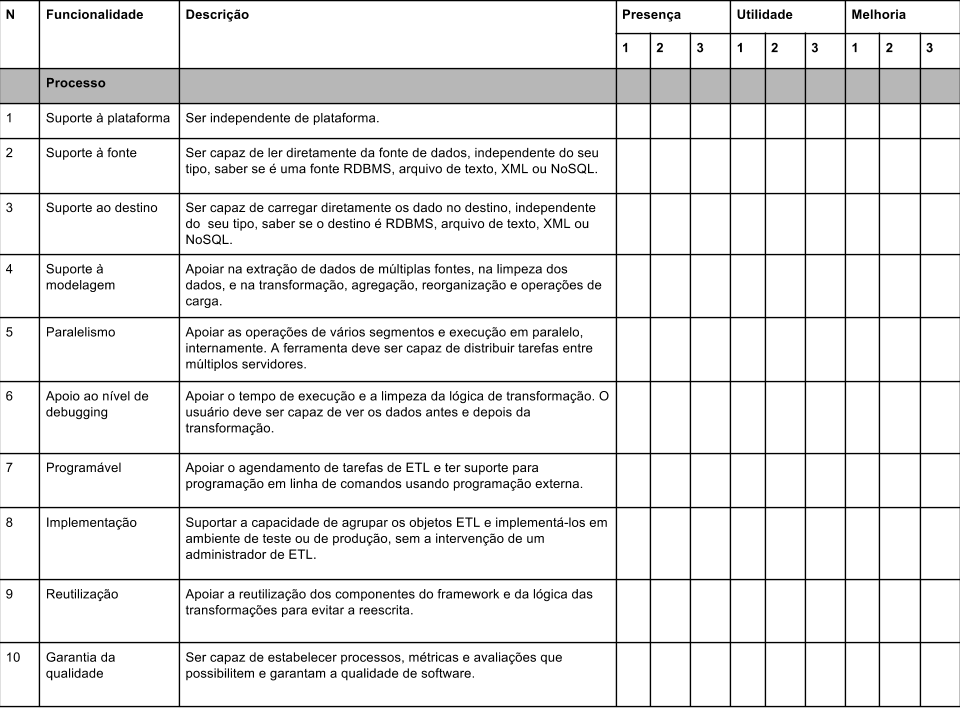
\includegraphics[scale=0.5]{fig/questionario_caracteristicas.png}
	\caption{Questionário de Funcionalidades}
	\label{questionariofuncionalidades}
\end{figure}

\clearpage

\subsection{Resultado do Estudo}


A figura \ref{presenca} apresenta o gráfico da quantidade de presença para cada funcionalidade de acordo com cada ferramenta de ETL. Já a figura \ref{utilidade} mostra o nível de importância que as ferramentas dão para cada funcionalidade e a figura \ref{melhoria} indica necessidade de melhorar funcionalidade em cada ferramenta.

\begin{figure}[h]
	\centering
	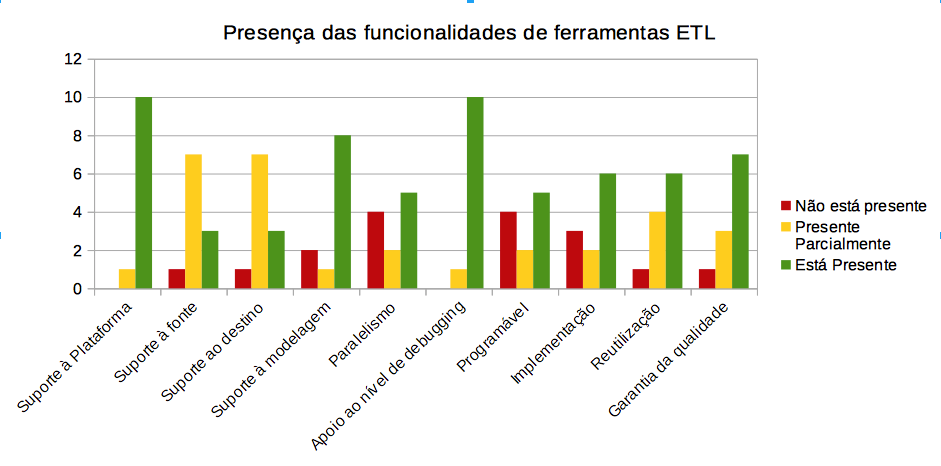
\includegraphics[scale=0.5]{fig/presenca.png}
	\caption{Quantidade de Presença para cada funcionalidade}
	\label{presenca}
\end{figure}

\begin{figure}[h]
	\centering
	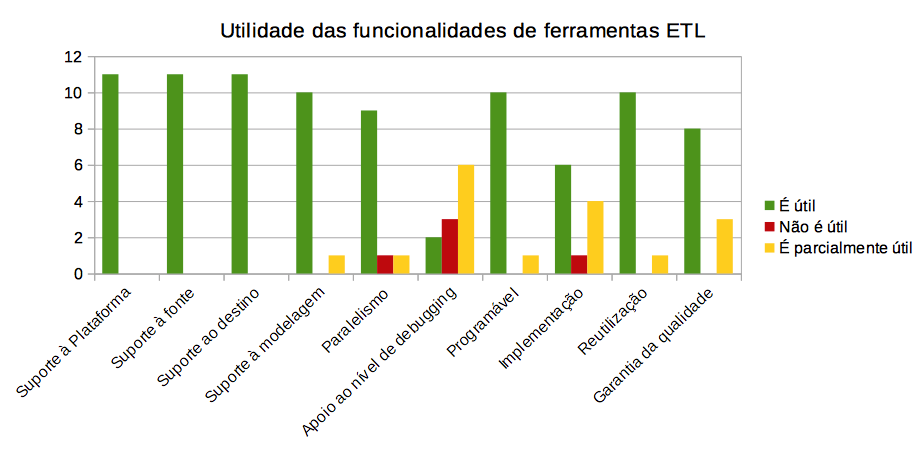
\includegraphics[scale=0.5]{fig/utilidade.png}
	\caption{Níveis de utilidade para cada funcionalidade}
	\label{utilidade}
\end{figure}

\begin{figure}[h]
	\centering
	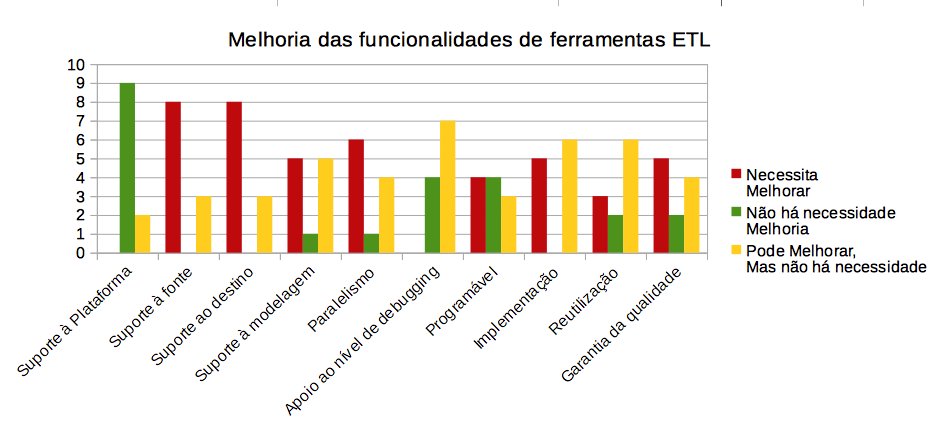
\includegraphics[scale=0.5]{fig/melhorias.png}
	\caption{Necessidade de melhoria para cada funcionalidade}
	\label{melhoria}
\end{figure}

\clearpage

O perfil dos participantes é apresentado no quadro \ref{resultadoperfil}, bem como a legenda para leitura do resultado.

\begin{table}
	\centering
	\caption{Resultado do Perfil dos participantes}
	\label{resultadoperfil}
\resizebox{\textwidth}{!}{\begin{tabular}{|r|r|r|r|r|r|r|r|r|r|}
		\hline
		Ferramenta & Código Fonte & Marca de mercado & Para NoSQL & GUI & Programável & Integrada & Processamento & Extensível & Finalidade\\
		\hline
		PygramETL  & 1 & 2 & 2 & 2 & 1 & 1 & 2 & 1 & 2 \\
		\hline
		
		
		
	\end{tabular}}
\end{table}
% ---
\section{Descrição}
\section{Considerações Finais}
